\documentclass[a4paper]{article}
\usepackage{import}
\usepackage{graphicx}
\usepackage{float}
\usepackage{pgfplots}
\usepackage{listings}
\usepackage{enumitem}
\usepackage{textcomp}
\usepackage{tikz}
\usetikzlibrary{decorations.pathreplacing} % for angle arc
\usetikzlibrary{angles, quotes, calc, positioning, trees} % for drawing angles
\pgfplotsset{compat=1.18,width=10cm}
\usepackage{tikz-cd}
\usepackage{booktabs}
\usepackage{cancel}
\usepackage{amsmath}
\usepackage{minted}
\usepackage{csquotes}
\usepackage{gensymb}
\usepackage{forest}
\usepackage{amsthm}
\usepackage{amssymb}
\usepackage{fontawesome} 
\usepackage{varwidth}
\usepackage{pgfplots}
\usepackage{lipsum}
\usepackage{mdframed} 
\usepackage{color}   
\usepackage{hyperref}
\newmdtheoremenv{theo}{Theorem}
\usepackage{mathtools}
\DeclarePairedDelimiter\ceil{\lceil}{\rceil}
\DeclarePairedDelimiter\floor{\lfloor}{\rfloor}

\hypersetup{
    colorlinks=true, %set true if you want colored links
    linktoc=all,     %set to all if you want both sections and subsections linked
    linkcolor=black,  %choose some color if you want links to stand out
}

% Define theorem styles
\newtheorem{theorem}{Theorem}[section]    % Theorems numbered within sections
\newtheorem{lemma}[theorem]{Lemma}        % Lemmas use the same counter as theorems
\newtheorem{corollary}[theorem]{Corollary} % Corollaries use the same counter as theorems
\newtheorem{proposition}[theorem]{Proposition} % Proposition uses the same counter
\newtheorem{property}[theorem]{Property}
\theoremstyle{definition}
\newtheorem{definition}[theorem]{Definition} % Now uses the same counter as theorems


% Remark-style theorem
\theoremstyle{remark}
\newtheorem{remark}[theorem]{Remark}

% Boxed environment for theorems
\newmdenv[
  linewidth=0.8pt,
  roundcorner=5pt,
  linecolor=black,
  backgroundcolor=white!5,
  skipabove=\baselineskip,
  skipbelow=\baselineskip,
  innerleftmargin=10pt,
  innerrightmargin=10pt,
  innertopmargin=5pt,
  innerbottommargin=5pt
]{thmbox}

% Custom proof environment (also boxed)
\renewenvironment{proof}[1][Proof]{%
  \begin{mdframed}[linewidth=0.8pt, roundcorner=5pt, linecolor=black, skipabove=\baselineskip, skipbelow=\baselineskip, innertopmargin=5pt, innerbottommargin=5pt]%
  \noindent\textbf{#1. }%
}{%
  \end{mdframed}%
}

% Redefine theorem environments to use thmbox
\let\oldtheorem\theorem
\renewenvironment{theorem}{\begin{thmbox}\begin{oldtheorem}}{\end{oldtheorem}\end{thmbox}}

\let\oldlemma\lemma
\renewenvironment{lemma}{\begin{thmbox}\begin{oldlemma}}{\end{oldlemma}\end{thmbox}}

\let\oldcorollary\corollary
\renewenvironment{corollary}{\begin{thmbox}\begin{oldcorollary}}{\end{oldcorollary}\end{thmbox}}

\let\oldproposition\proposition
\renewenvironment{proposition}{\begin{thmbox}\begin{oldproposition}}{\end{oldproposition}\end{thmbox}}

\let\oldproperty\property
  \renewenvironment{property}{\begin{oldproperty}}{\end{oldproperty}}


% Reference shortcuts
\newcommand{\thmref}[1]{Theorem~\ref{#1}}
\newcommand{\lemref}[1]{Lemma~\ref{#1}}
\newcommand{\corref}[1]{Corollary~\ref{#1}}
\newcommand{\propref}[1]{Property~\ref{#1}} 

% To customize QED symbol
\renewcommand{\qedsymbol}{$\blacksquare$}

\usetikzlibrary{decorations.pathreplacing} % for angle arc
\usetikzlibrary{angles, quotes, calc} % for drawing angles

\usepackage{color}   %May be necessary if you want to color links
\usepackage{hyperref}
\hypersetup{
    colorlinks=true, %set true if you want colored links
    linktoc=all,     %set to all if you want both sections and subsections linked
    linkcolor=black,  %choose some color if you want links to stand out
}

\usepackage{xcolor}
\usepackage[most]{tcolorbox}


% Define a custom tcolorbox environment for examples
\newtcolorbox{examplebox}[2][]{
  colback=blue!5!white,
  colframe=blue!30!black,
  title=#2,
  boxrule=0mm,
  fonttitle=\bfseries,
  width=\textwidth,
  breakable,
  #1
}

\newtcolorbox{definizione}[2] {
  colback=green!5!white,
  colframe=green!30!black,
  title=#2,
  boxrule=0mm,
  fonttitle=\bfseries,
  width=\textwidth,
  breakable,
  #1
}

\definecolor{codegreen}{rgb}{0,0.6,0}
\definecolor{codegray}{rgb}{0.5,0.5,0.5}
\definecolor{codepurple}{rgb}{0.58,0,0.82}
\definecolor{backcolour}{rgb}{0.95,0.95,0.92}

\lstdefinestyle{mystyle}{
    backgroundcolor=\color{backcolour},   
    commentstyle=\color{codegreen},
    keywordstyle=\color{magenta},
    numberstyle=\tiny\color{codegray},
    stringstyle=\color{codepurple},
    basicstyle=\ttfamily\footnotesize,
    breakatwhitespace=false,         
    breaklines=true,                 
    captionpos=b,                    
    keepspaces=true,                 
    numbers=left,                    
    numbersep=5pt,                  
    showspaces=false,                
    showstringspaces=false,
    showtabs=false,                  
    tabsize=2
}

\lstset{style=mystyle}

\makeatletter
\renewcommand*\env@matrix[1][*\c@MaxMatrixCols c]{%
  \hskip -\arraycolsep
  \let\@ifnextchar\new@ifnextchar
  \array{#1}}
\makeatother


\onehalfspacing
\title{Fondamenti di Informatica}
\author{Università di Verona\\Imbriani Paolo - VR500437\\Professor Isabella Mastroeni}

\begin{document}

\begin{figure}
    \centering
    
\includegraphics[width=0.3\textwidth]{../UniversityofVerona.png}
    \label{fig:centered-image}
\end{figure}

\maketitle

\pagebreak

\tableofcontents

\pagebreak

\section{Cosa è l'informatica?}

La domanda chiave di questo corso è: \textit{``Cosa è l'informatica?''}. 
Ci sono diversi definizioni a seconda del contesto, ma in generale l'informatica è lo studio dei processi che trasformano l'informazione.
Possiamo vedere, storicamente, diverse definizioni come quella in inglese come "Computer Science" che vede
l'informatica come studio della calcolabilità, della computazione e dell'informazione.

\subsection{Perché la calcolabilità}

Si studia la calcolabilità perché ci aiuta a capire cosa possiamo fare con gli strumenti che abbiamo.
Quando descriviamo un programma, quanto tempo ci mette e quanto spazio utilizza è una domanda importante 
per capire se il programma è efficiente o meno. Anche in senso dei linguaggi di programmazione per capire se usiamo
quello giusto per il problema che stiamo cercando di risolvere. Chiaramente è un qualcosa che in continuo
sviluppo perché si evolve in base alla tecnologia che abbiamo a disposizione.
\\
\\
Uno dei pionieri è stato \textbf{Hilbert} che si chiedeva se la matematica fosse formalizzabile come insieme
finito (non contraddittorio) di assiomi? Godel dimostrò che non è possibile rappresentare la matematica 
come un insieme finito di assiomi in maniera non contradditoria, dicendo che in ogni sistema formale
ci sono proposizioni vere che non possono essere dimostrate all'interno del sistema.
\\
\\
Nel tentativo di rispondere a queste (ed altre) domande si è costruito un modello che 
permette di comprendere profondamente ilr agionamento computazionale,
permettendo di applicarlo ad ogni disciplina.
Cosa è calcolabile e cosa non lo è? 

\subsubsection{Macchina di Turing} 

Anche Turing si pose questa domanda e propose la \textbf{Macchina di Turing} come modello di calcolo.
Una sola macchina (programmabile) per tutti i problemi.
La macchina è universale (interprete):
\[Init(P,x)\ = \begin{cases}
    P(x) & \text{se } P \text{ è un programma che termina}\\
    \uparrow & \text{se } P \text{ è un programma che non termina}
\end{cases}\]
Se un problema è intuitivamente calcolabile, allora esisterà una macchina di Turing (o un dispostivo
equivalente, come il computer) in grado di risolverlo, cioè calcolarlo.
I modelli equivalenti possono essere:
\begin{itemize}
    \item Lambda calcolo 
    \item Funzioni ricorsive
    \item Linguaggi di programmazione (Turing completi)
\end{itemize}
I problemi non calcolabili sono infinitamente più numerosi di quelli calcolabili.
\subsubsection{Limiti dell'informatica}

L'informatica ha più limiti di quanto si possa pensare, definiti dall'equivalenza di Turing
e l'incompletezza di Godel che ci dicono che non possiamo risolvere tutti i problemi.
Ci sono anche limiti fisici e tecnologici come:
\begin{itemize}
    \item Dati non osservabili (teorema di Shannon)
    \item Dati non controllabili (velocità della luce)
\end{itemize}

\subsection{Basi di logica}

Alcune nozioni di logica che ci serviranno in seguito:

\begin{itemize}
    \item \textbf{Linguaggio del primo ordine:} 
    \begin{itemize}
        \item Simboli relazionali $(p,q, ...)$
        \item Simboli di funzione $(f,g, ...)$
        \item Simboli di costante $(c,d, ...)$
    \end{itemize}
    \item \textbf{Simboli logici:}
    \begin{itemize}
        \item Parentesi (,) e virgola
        \item Insieme numerabile di variabili $(v,x,...)$
        \item Connettivi logici ($\neg, \land, \lor, \rightarrow, \leftrightarrow$)
        \item Quantificatori ($\forall, \exists$)
    \end{itemize}
    \item \textbf{Termini:}
        \begin{itemize}
            \item Variabili
            \item Costanti
            \item $f$ simbolo di funzione m-ario $t_1, t_2, \dots, t_m$ termini, allora $f(t_1, t_2, \dots, t_m)$ è un termine.
        \end{itemize}
    \item \textbf{Formula atomica:} $p$ simbolo di relazione n-ario, 
    $t_1,t_2,\dots,t_n$ 
    termini, allora $p(t_1,t_2,\dots,t_n)$ è una formula atomica.
    \item \textbf{Formula:}
    \begin{itemize}
        \item Formula atomica
        \item $\phi$ formula, allora $\neg \phi$ è una formula
        \item $\phi$ e $\psi$ formule, allora $(\phi \land \psi)$, $(\phi \lor \psi)$, $(\phi \rightarrow \psi)$, $(\phi \leftrightarrow \psi)$ sono formule.
        \item $\phi$ formula e $v$ variabile, alloar e $\forall v . \phi$ e $\exists v . \phi$ sono formule.
    \end{itemize}
\end{itemize}

\subsection{Nozioni sugli insiemi}

\begin{itemize}
    \item $x \in A$ signfiica che $x$ è un elemento dell'insieme $A$
    \item $\{x | P(x)\}$ si identifica insieme costuito dagli $x$ che soddisfano la proprietà (o predicato) $P(x)$
    \item $A \subseteq B$ significa che $A$ è un sottoinsieme di $B$ se ogni elemento di $A$ è anche in $B$
    \item $\mathcal{P}(S)$ denota l'insieme delle parti di $S$, ovvero l'insieme di tutti i sottoinsiemi di $S$ ($\mathcal{P}(S) = \{X | X \subseteq S\}$)
    \item $A \backslash B = \{x | x \in A \land x \notin B\}, A \cup B = \{x | x \in A \lor x \in B\}, A \cap B = \{x | x \in A \land x \in B\}$   
    \item $|A|$ denota la cardinalità di $A$, ovvero il numero di elementi in $A$.
    \item $\bar{A}$ denota il complemento di $A$, ovvero $x \bar{\in} A \leftrightarrow x \notin A$
\end{itemize}

\subsection{Nozioni sulle relazioni}

\begin{itemize}
    \item Prodotto cartesiano: $A_1 \times A_2 \times \dots \times A_n = \{\langle a_1,a_2,\dots,a_n \rangle | a_1 \in A_1,\dots, a_n \in A_n\}$
    \item Una \textbf{RELAZIONE} (binaria) è un sottoinsieme del prodotto cartesiano di (due) insiemi; dati $A$ e $B$, $R \subseteq A \times B$ 
    è una relazione su $A$ e $B$ 
    \begin{itemize}
        \item \textbf{Riflessiva:} $\forall a \in S$ si ha che $aRa$
        \item \textbf{Simmetrica:} $\forall a,b \in S$ se $aRb$ allora $bRa$
        \item \textbf{Antisimmetrica:} $\forall a,b \in S$ se $aRb$ e $bRa$ allora $a=b$
        \item \textbf{Transitiva:} $\forall a,b,c \in S$ se $aRb$ e $bRc$ allora $aRc$
    \end{itemize}  
    \item Per ogni relazione $R \subseteq S \times S$ la chiusura transitiva di $R$ è il più piccolo 
    insieme $R^*$ tale che $\langle a,b \rangle \in R \land \langle b,c \rangle \in R \rightarrow \langle a,c \rangle \in R^*$  
    \item Una relazione è detta \textbf{totale} su $S$ se $\forall a,b \in S$ si ha che $aRb \lor bRa$
    \item Una relazione $R$ di \textit{di equivalenza} è una relazione binaria riflessiva, simmetrica e transitiva.
    \item Una relazione binaria $R \subseteq S \times S$ è un \textbf{pre-ordine} se è riflessiva e transitiva.
    \item $R$ è un ordine parziale se è un pre-ordine antisimmetrico.
    \item $x \in S$ è \textbf{minimale} rispetto a $R$ se $\forall y \in S . y \not{R} x$ (ovvero $\neg(yRx))$
    \item $x \in S$ è \textbf{minimo} rispetto a $R$ se $\forall y \in S . xRy$
    \item $x \in S$ è \textbf{massimale} rispetto a $R$ se $\forall y \in S . x \not{R} y$ (ovvero $\neg(xRy)$)
    \item $x \in S$ è \textbf{massimo} rispetto a $R$ se $\forall y \in S . yRx$
\end{itemize}

\subsection{Nozioni sulle funzioni}

\begin{itemize}
    \item Una relazione $f$ è una \textbf{funzione} se $\forall a \in A$ esiste uno ed un solo $b \in B$ tale che $(a,b) \in f$
    \item $A$ dominio e $B$ codominio di $f$. Il range di $f$ è l'insieme di tutti i valori che $f$ può assumere.
    \item f è \textbf{iniettiva} se $\forall a_1,a_2 \in A$ se $a_1 \neq a_2$ allora $f(a_1) \neq f(a_2)$
    \item Se $f : A \mapsto B$ è sia iniettiva che suriettiva allora è \textbf{biiettiva} e quindi esiste $f^{-1} : B \mapsto A$ 
\end{itemize}



\section{Funzioni calcolabili}

Un insieme è a tutti gli effetti una proprietà che dato un oggetto
stabilisce se esso all'interno di insieme o no.
\[\text{Problemi} \equiv \text{Funzioni} \; \; f : \mathbb{N} \rightarrow \mathbb{N}\]
Ci chiediamo se questa funzioni siano tutte calcolabili (intuitivamente). Da il teorema che abbiamo citato
nei precedenti paragrafi (quello dell'incompletezza) sappiamo che non è così.
Cerchiamo di vedere insiemisticamente perché questo è giustificato.

\dfn{Intuitivamente Calcolabile}
{
Qualcosa che è \textbf{intuitivamente calcolabile} è qualcosa è che riusciamo a descrivere
attraverso un algoritmo, ovvero una sequenza finita di passi discreti elementari.
}
La funzione di tipo:
\[f : \mathbb{N} \rightarrow \mathbb{N}\]
è un \textbf{insieme} di associazioni input-output. 
\ex{}
{
    \[
    \begin{aligned}
        f = \text{quadrato} &= \{(0,0), (1,1), (2,4), (3,9), (4,16), ...\} \\
        &= \{(x,x^2) \; | \; n \in \mathbb{N} \} \\
    \end{aligned}   \]
    Quindi $f$ è un insieme di coppie in $\mathbb{N} \times \mathbb{N}$.
    Quindi $|\mathbb{N} \times \mathbb{N}| = |\mathbb{N}|$ (cardinalità di $\mathbb{N} \times \mathbb{N}$
    Quindi
    \[f \subseteq \mathbb{P}(\mathbb{N} \times \mathbb{N}) = \mathbb{P}(\mathbb{N})\]
    Per esempio se:
    \[A=\{1,2,3\} \text{ allora } \mathbb{P}(A) = \{\emptyset, \{1\}, \{2\}, \{3\}, \{1,2\}\}\]
    dove $|\mathbb{P}(A)| = 2^{|A|}$. 
    \[|\mathbb{N}| = \omega < |P(\mathbb{N})|) = |\mathbb{R}|\]
    e quindi l'insieme delle funzioni \textbf{non è numerabile}.
}
\subsection{Quale funzioni numerabili ci sono?}
$\Sigma = $alfabeto finito di simboli che uso per il programma/algoritmo
\[\Sigma = {s_1, s_2, s_3, \dots}\] 
quindi un programma non è nient'altro che un sottoinsieme finito di $\Sigma^*$ (tutte le stringhe finite che posso formare con l'alfabeto).
\[\Sigma = {a,b,c}\]
\[\Sigma^* = \{\emptyset, a,b,c,ab,ba,ac,cd,bc,cb,\dots\}\]
in questo caso, la sequenza di simboli in $\Sigma^*$ è numerabile, perché
\[|\Sigma^*| = |\mathbb{N}|\]
\[|\text{Programmi in }\mathbb{N}| = |\Sigma^*| = |\mathbb{N}|\]
e di conseguenza l'insieme dei programmi è numerabile.
Una veloce constatazione che possiamo fare è vedere quindi che l'insieme delle funzioni 
calcolabili è numerabile, perché ogni funzione calcolabile 
è associata ad almeno un programma che la calcola.

\begin{figure}[H]
    \centering
    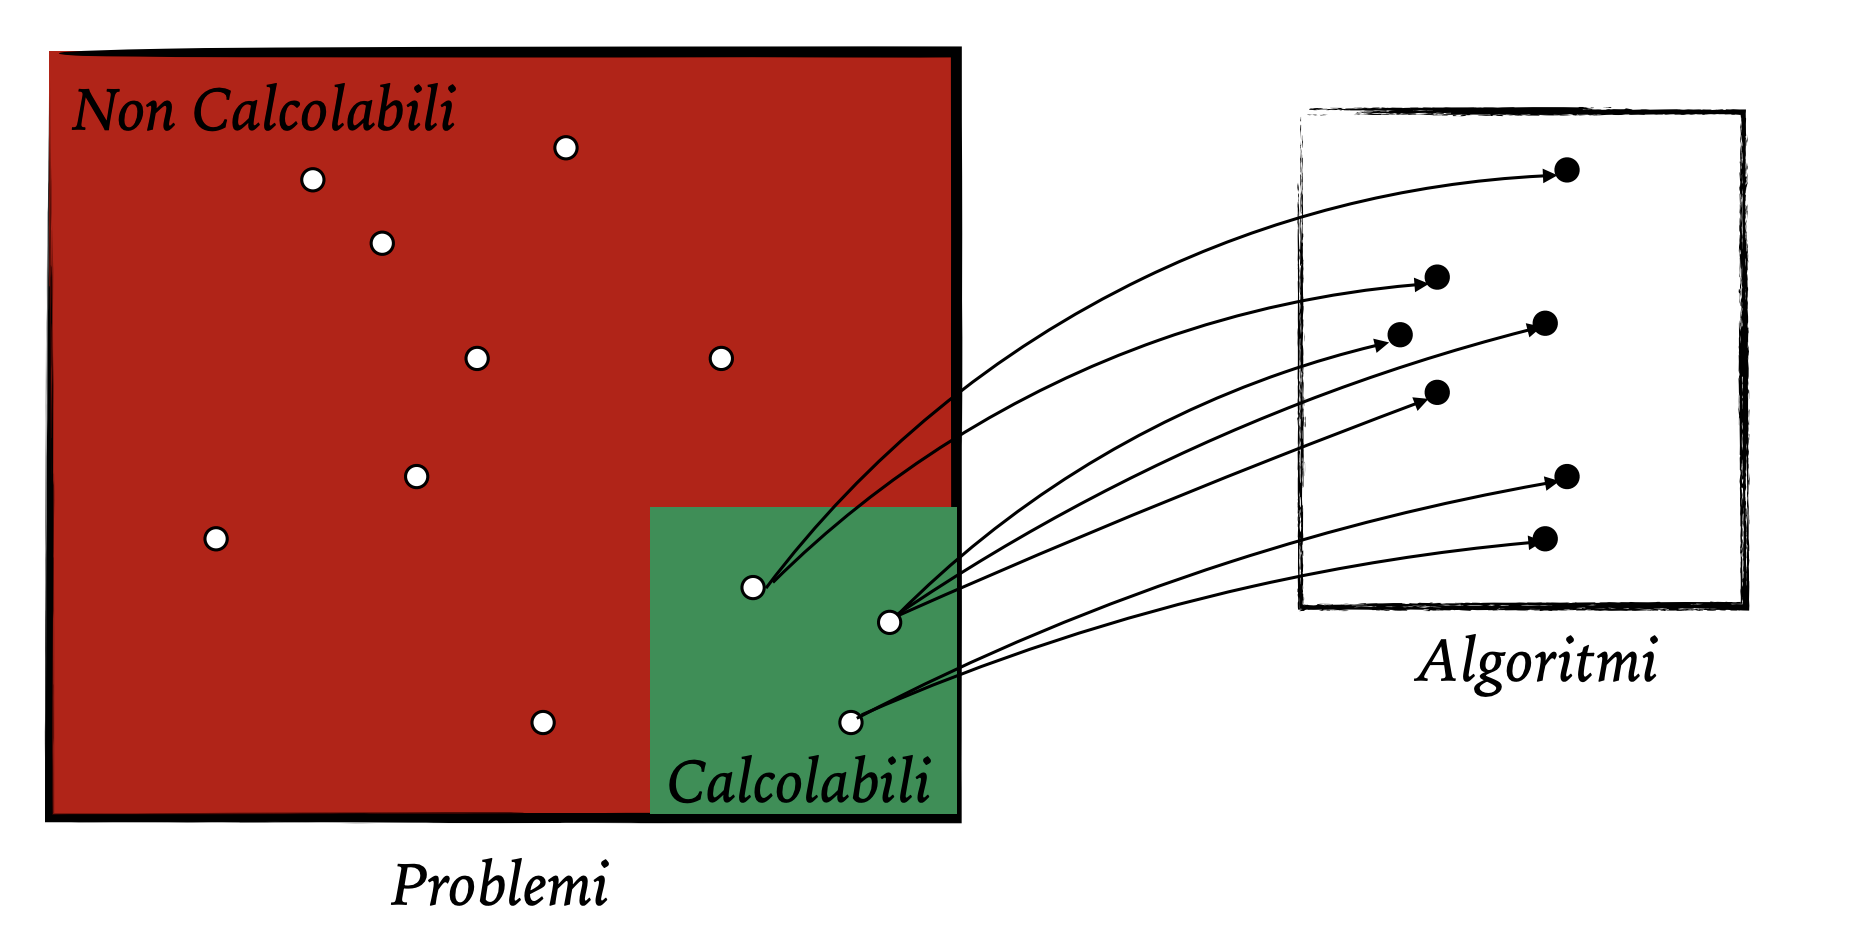
\includegraphics[width=0.9\textwidth]{fcalcolabili.png}
\end{figure}

\section{Principio di induzione}

Il principio di induzione ha senso solo su insieme infiniti 
e serve per dimostrare che una proprietà vale per tutti gli elementi.
Esistono due metodi di induzione:
\begin{itemize}
    \item Induzione matematica
    \item Induzione strutturale
\end{itemize}
Tratteremo nello specifico caso in questo corso \textbf{l'induzione matematica.}
Partiamo da un insieme $A$ infinito con una relazione $< \; : (A, <)$ è una relazione d'ordine
non riflessiva perché non è minore stretto.
Utilizziamo l'induzione matematica e quindi $A = \mathbb{N}$ e $<$ 
è l'ordinamento stretto tra numeri. Una relazione d'ordine deve essere
\textit{ben fondata} vuol dire che non esistono catene discendenti infinite.
Una catena discendente è una sequenza infinita di elementi
\[a_0 > a_1 > a_2 > a_3 > \dots\]
In un tipo di relazione riflessiva è sicuramente non ben fondata perché posso fare 
continuare ad inserire lo stesso numero all'infinito.
\[m \text{ minimale in } A \; : \; b \in A \text{ è minimale se } \forall b' < b . b' \notin A\]
\ex{}
{
    Se prendiamo $\{1,2,3\}$ con relazione d'ordine di contenimento
    allora esistono più minimali come $\{1,2\}$ o $\{2,3\}$. 
    Quindi se $A = \mathbb{N} \Longrightarrow \exists b $ minimo $\forall x \subseteq \mathbb{N}$. 
}
\noindent
Quindi preso $A$ insieme ben fondato con ordinamento $<$ allora:
$\pi$ proprietà definita sugli elementi di \[
A: \pi \subseteq A \text{ allora } 
\forall a \in A \, .\pi(a) \Longleftrightarrow \forall a \in A . [[\forall b < a . \pi(b)] \rightarrow \pi(a)]
\]
Se dimostriamo $\pi$ per ogni elemento più piccolo di $a$ allora $\pi$ vale per $a$.
\[{Base}_A = \{a \in A | a \text{ minimale}\}\]
Quindi
\[\overbrace{\forall A \in {Base}_A \; . \; \pi(a)}^{\text{Base}} \; \and \; 
\underbrace{\forall a \in A . {Base}_A}_{\text{passo induttivo}} . \overbrace{\forall b < a . \pi(b)}^{\text{ipotesi induttiva}} \rightarrow \underbrace{\pi(a)}_{\text{tesi}}
\]
\ex{}
{
    Prendiamo come esempio il seguente enunciato:
    \[\forall n \in \mathbb{N}, \; \;  \sum_{i = 1}^{n} i = \frac{n(n+1)}{2}\]
    \textbf{Base:} $n=1$
    \[A = \mathbb{N} \backslash \{0\} \; \; {Base}_A = \{1\} \rightarrow \sum_{i=1}^{1} i = 1\]
    \[
    \begin{aligned}
        \sum_{i=1}^{1} i &= 1\\
        &= n(n+1)/2\\
        &= \frac{1(1+1)}{2} = 1\\
    \end{aligned}    
    \]
    Caso base dimostrato.\\
    \textbf{Passo induttivo:} prendo $n \in \mathbb{N}$ e applico l'ipotesi induttiva: per ogni $k < n$ vale la tesi.
    \[\text{ Tesi da dimostrare: } \sum_{i=1}^{n} i = \frac{n(n+1)}{2}\]
    \[\sum_{i=1}^{n} i = \sum_{i=1}^{n-1}i + n\]
    Sappiamo sicuramente che $n-1 < n$ e per ipotesi induttiva:
    \[\sum_{i=1}^{n-1}i + n= \frac{(n-1)(n-1+1)}{2} + n = \frac{n(n-1)}{2} + n = \]
    \[\frac{n(n-1) + 2n}{2} = \frac{n(n-1+2)}{2} = \frac{n(n+1)}{2} \quad \square\] 
    e quindi la tesi vale perché siamo arrivati alla stessa espressione
    che volevamo dimostrare.
}
\subsection{Linguaggi formali}
\dfn{Linguaggio formale}
{
    Un linguaggio formale è un insieme di stringhe composte da simboli in un alfabeto finito $\Sigma$.
}
\noindent
$\Sigma^*$ denota il linguaggio di tutte le stringhe dell'alfabeto $\Sigma$, se $\Sigma$ non è vuota allora $\Sigma^*$ è 
infinito e numerabile.
Solitamente un linguaggio formale $\mathcal{L}$ è un sottoinsieme di $\Sigma^*$ tipicamente infiniti ma non è necessario:
\[\mathcal{L} \subseteq \Sigma^*\]
I linguaggi finiti sono sicuramente regolari perché \textit{posso sempre costruire un automa a stati finiti} che li riconosce.

\begin{figure}[H]
    \centering
    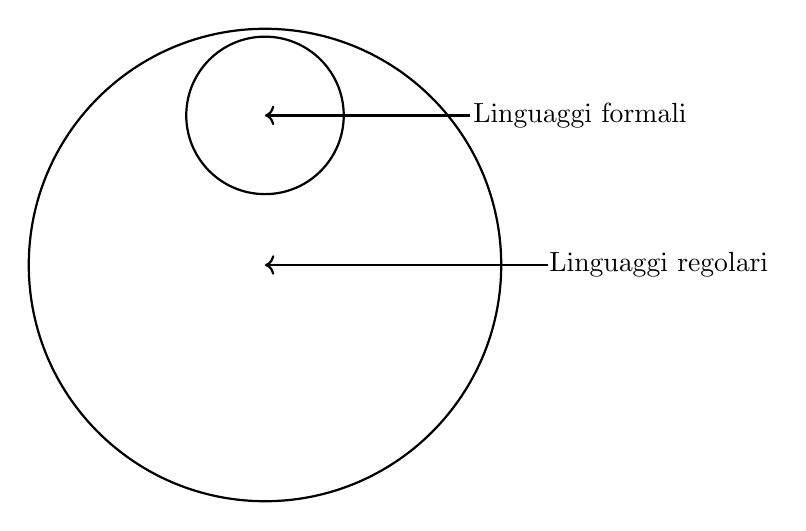
\begin{tikzpicture}
        \draw[thick] (0,0) circle(3);
        \draw[thick] (0,1.9) circle(1);
        \node at (4,1.9) {Linguaggi formali};
        \draw[<-, thick] (0,1.9) -- (2.6,1.9);
    
        \node at (5,0) {Linguaggi regolari};
        \draw[<-, thick] (0,0) -- (3.6,0);
      \end{tikzpicture}
\end{figure}


\begin{figure}[H]
    \centering
    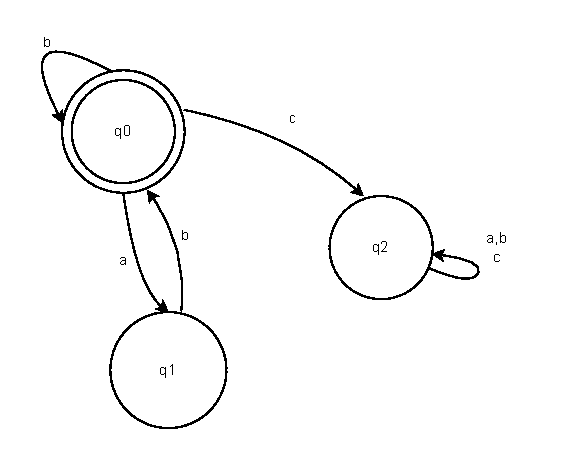
\includegraphics[width=0.6\textwidth]{automa.pdf}
    \caption{Esempio di automa a stati finiti}
\end{figure}
\noindent
Come abbiamo detto in precedenza, una funzione è \textit{calcolabile}
se possiamo pensare ad un algoritmo per calcolarla.
Tra le funzioni calcolabili, ci sono quelle totali, ovvero quelle che terminano per ogni input.
\ex{}
{
    Pensiamo ad una funzione $f \subseteq \mathbb{N} \times \mathbb{N}$,
    la possiamo descrivere come associazione di coppie:
    \[f(0) = 1, f(1) = 1, f(2) = 2, f(3) = 3, f(4) = 5, f(5) = 8, \dots\]
    Tuttavia servirebbe scrivere una quantità infinita di coppie per descrivere la funzione.
    Quindi proviamo a farlo ma stavolta ricorsivamente.
    \[
    \begin{cases}
        f(0) = 1 = f(1)\\
        f(x+2) = f(x+1) + f(x)
    \end{cases}
    \]
}

\subsection{Funzioni e insiemi}

In realtà ci sta un forte legame tra funzioni e insiemi perché per esempio dovessimo prendere una funzione
$f : \mathbb{N} \rightarrow \mathbb{N}$, questa funzione può essere vista come un linguaggio $L_f = \{1^{f(x)} | x \in \mathbb{N}\}$ 
che è l'insieme delle stringhe composte da $f(x)$ simboli 1.
Il nostro linguaggio $\Sigma = \{1\}$ e quindi il linguaggio è un sottoinsieme di $\Sigma^*$.
Il nostro linguaggio ci può dire se un oggetto in input fa parte o no dell'insieme.
Parliamo di \textbf{insiemi} invece che di funzioni
dove gli elementi dell'insieme dipendono dal calcolo della funzione.
\ex{}
{
    Se io dovessi scrivere una funzione costante del tipo $f(x) = 2$.
    In questo caso riconosciamo che il linguaggio $L_f$ è finito perché
    \[L_f = \{1\}\]
    L'unica combinazione possibile è una singola stringa.
    Il linguaggio si dice finito che è sottoinsieme di linguaggi totali.
}
\ex{}
{
    In questo caso la funzione $f(x) = 2x$ è una funzione lineare.
    Ho bisogno di una memoria finita. Mi sposto tra queste informazioni per
    determinare se la stringa in input fa parte o no del linguaggio.
    Questa funzione è anche detta \textbf{regolare}.
}
\ex{}
{
    $f(\sigma) = \sigma_{\text{reverse}}$ quindi per esempio:
    \[f(abc) = cba\]
    Tuttavia per questa funzione non mi basta più una memoria finita ma
    illimitata essendo che non posso sapere a priori quanta memoria abbia bisogno la funzione
    (è sufficiente uno stack).
    Questo tipo di funzione è detta anche \textbf{context free}.
}
\ex{}
{
    Nel caso di $f(x) = x^2$ sappiamo sicuramente
    che possiede un output preciso ma avrei bisogno di una memoria illimitata per rappresentarla.
}

\section{Linguaggi Regolari}

\subsection{Automa a stati finiti determinsitici (DFA)}

Quando parliamo di memoria è facilmente codificabile 
in termini di stati. Dal punto di vista grafico possiamo rappresentarli
come nodi collegati da archi.
Prendiamo per esempio il linguaggio $L_f$ di prima:
\[L_f = \{1^{2n} \; | \; n \in \mathbb{N}\}\]
\[\Sigma = {1}\]

\begin{figure}[H]
    \centering
    \begin{tikzpicture}[node distance = 3cm, on grid, auto]
    
      \node[state, initial, accepting] (q0) {$q_0$};
      \node[state, right of = q0] (q1) {$q_1$};
      \draw (q0) edge[bend left, above] node{1} (q1);
    \draw (q1) edge[bend left, below] node{1} (q0);
    \end{tikzpicture}
  \end{figure}

\dfn{Automa a stati finiti}
{
    \[M = (Q, \Sigma, \delta, q_0, F)\]
    è un automa a stati finiti deterministico dove:
    \begin{itemize}
        \item $Q$ è un insieme finito di stati (ogni stato rappresenta "un informazione")
        \item $\Sigma$ è un alfabeto finito di simboli
        \item $\delta : Q \times \Sigma \rightarrow Q$ è la funzione di transizione (descrive come evolve il
        calcolo a partire dallo stato raggiunto e dal simbolo letto)
        \item $q_0 \in Q$ è lo stato iniziale
        \item $F \subseteq Q$ è l'insieme di stati finali (o di accettazione)
    \end{itemize}
}
\begin{table}[H]
    \centering
    \begin{tabular}{|c|c|c|}
        \hline
        $\Sigma \backslash Q$ & $q_0$ & $q_1$\\
        \hline
        1 & $q_1$ & $q_0$ \\
        \hline
    \end{tabular}
\end{table}
\noindent
Ci sta poi la funzione $\hat{\delta} : Q \times \Sigma^* \rightarrow Q$ che estende la funzione di transizione e descrive
lo stato che raggiungiamo leggendo una sequenza di simboli.
\[
\begin{cases}
    \hat{\delta}(q, \epsilon) = q\\
    \hat{\delta}(q, w a) = \hat{\delta}(\delta(q,w), a)
\end{cases}
\quad w \in \Sigma^*, a \in \Sigma
\]
anche chiamata chiusura transitiva di $\delta$. Quindi mi permette
di calcolare lo stato raggiunto leggendo una stringa di simboli.

\subsection{Come si dimostra che un linguaggio è regolare?}

\ex{}
{
    Prendiamo come esempio il linguaggio:
    \[L = \{\sigma \; | \; \text{ $\sigma$ contiene almeno due 1}\}\]
    \[\Sigma = \{0,1\}\]
    Per esempio:
    \[110, 101, 111, 011, 1001 \in L\]
    \[0, 00, 000, 01, 10, 0000 \notin L\]
    Quindi intuitivamente come possiamo definire l'automa?
    \begin{figure}[H]
        \centering
        \begin{tikzpicture}[->, node distance = 3cm, on grid, auto]
        
          \node[state, initial] (q0) {$q_0$};
          \node[state, right of = q0] (q1) {$q_1$};
          \node[state, accepting, right of = q1] (q2) {$q_2$};


        \draw (q0) edge[bend left, above] node{1} (q1);
        \draw (q0) edge[loop above] node{0} (q0);
        \draw (q1) edge[loop above] node{0} (q1);
        \draw (q1) edge[bend left, above] node{1} (q2);
        \draw (q2) edge[loop above] node{0,1} (q2);
        \end{tikzpicture}
      \end{figure}
    \noindent
    Un linguaggio $L$ è riconosciuto da $M$ (Automa a stati finiti deterministico o DFA)
    se $L = L(M)$ dove $L(M)$ è il linguaggio di $n$ definito come:
    \[L(M) = \{\sigma \in \Sigma^* \; | \; \hat{\delta}(q_0, \sigma) \in F\}\]
    Sono tutte le stringhe che partendo da $q_0$ (stato iniziale) raggiunge uno stato finale.
}
\dfn{}
{
    Per dimostrare che $L$ è regolare dobbiamo costruire $M$ (almeno un $M$) e dimostrare che
    $L(M) = L$.
}
\[L = L(M) \equiv L \subseteq L(M) \text{ e } L(M) \subseteq L\]
\begin{enumerate}
    \item \[L \subseteq L(M) \equiv \sigma . \in L \rightarrow \sigma \in L(M)\]
    \[\sigma \in L \rightarrow \hat{\delta}(q_0, \sigma) \in F\]
    \item 
    \[
    \begin{aligned}
        L(M) \subseteq L &\equiv \sigma \in L(M) \rightarrow \sigma \in L\\
        & \hat{\delta}(q_0, \sigma) \in F \rightarrow \sigma \in L \equiv \\
        &\sigma \notin L \rightarrow \hat{\delta}(q_0, \sigma) \notin F
    \end{aligned}
    \]
\end{enumerate}
Dimostriamo per induzione sulla lunghezza delle stringhe $\sigma \in \Sigma^*$ che
se $\sigma \in L$ allora $\hat{\delta}(q_0, \sigma) \in F$
e $\sigma \notin L$ allora $\hat{\delta}(q_0, \sigma) \notin F$.
\ex{}
{
    \[L = \{\sigma \; | \; \text{ $\sigma$ contiene almeno due 1}\}\]
    \begin{figure}[H]
        \centering
        \begin{tikzpicture}[->, node distance = 3cm, on grid, auto]
        
          \node[state, initial] (q0) {$q_0$};
          \node[state, right of = q0] (q1) {$q_1$};
          \node[state, accepting, right of = q1] (q2) {$q_2$};


        \draw (q0) edge[bend left, above] node{1} (q1);
        \draw (q0) edge[loop above] node{0} (q0);
        \draw (q1) edge[loop above] node{0} (q1);
        \draw (q1) edge[bend left, above] node{1} (q2);
        \draw (q2) edge[loop above] node{0,1} (q2);
        \end{tikzpicture}
      \end{figure}
    \noindent
    Dimostriamo per induzione sulla lunghezza delle stringhe \( \sigma \in \Sigma^* \) 
  che se \( x \in L \) allora \( \hat{\delta}(q_0, x) \in F \) e se \( x \notin L \) allora
  \( \hat{\delta}(q_0, x) \notin F \).

  \vspace{1em}
  \noindent
  \( \left| \sigma  \right| = 0 \) non è \textbf{mai} sufficiente come base, ma
  è eventualmente la base \textbf{solo} per una delle due dimostrazioni. Bisogna
  quindi prendere la lunghezza più piccola che permette di avere sia \( \sigma \in L \) 
  che  \( \sigma \notin L \), in questo caso è \( \left| \sigma  \right| = 2 \).
  Per ogni \( \sigma  \) tale che \( \left| \sigma  \right| < 2 \quad \sigma \notin L \)
  perchè non può contenere due 1 e non è riconosciuta da \( M \) dove il primo stato finale
  è raggiunto leggendo almeno due simboli.
  \[
    \varepsilon \in L \quad \varepsilon \notin L
  \] 
  \begin{itemize}
    \item \textbf{Base}: Controlliamo ogni stringa di lungheezza minima nel linguaggio per
      provare il caso base
      \[
        \begin{cases}
          \sigma &= 11 \in L \; \text{ e } \; \hat{\delta}(q_0, 11) = q_2 \in F \\
          \sigma &= 10 \notin L \; \text{ e } \; \hat{\delta}(q_0, 10) = q_1 \notin F \\
          \sigma &= 01 \notin L \; \text{ e } \; \hat{\delta}(q_0, 01) = q_1 \notin F \\
          \sigma &= 00 \notin L \; \text{ e } \; \hat{\delta}(q_0, 00) = q_0 \notin F
        \end{cases}
      \] 

    \item \textbf{Passo induttivo}: Dimostriamo l'\textbf{ipotesi induttiva}, cioè
      la tesi con un limite fissato:
      \[
        \forall \sigma \in \Sigma^* \;.\; \left| \sigma  \right| \le n \;.\;
        \begin{cases}
          \sigma \in L &\Rightarrow \hat{\delta}(q_0, \sigma) \in F\\
          \sigma \notin L &\Rightarrow \hat{\delta}(q_0, \sigma) \notin F
        \end{cases}
      \] 
      Vogliamo dimostrare se \( \left| \sigma  \right| = n + 1 \) (la successiva stringa
      che posso considerare) allora vale
      \( 
        \begin{cases}
          \sigma \in L \Rightarrow \hat{\delta}(q_0,\sigma) \in F\\
          \sigma \notin L \Rightarrow \hat{\delta}(q_0,\sigma) \notin F
        \end{cases}
      \) 

      \vspace{1em}
      \noindent
      Dimostrazione:
      \[
        \left| \sigma  \right| = n + 1 \to 
          \sigma = \sigma'1 \; \vee \; \sigma = \sigma'0
      \] 
      \begin{itemize}
        \item Supponiamo che \( \sigma  \) appartiene al linguaggio e termini con 1:
          \[
            \sigma \in L \wedge \sigma  = \sigma'1 \to 
          \] 
          \begin{itemize}
            \item Se \( \sigma' \in L \) applico l'ipotesi induttiva:
              \[
                  \hat{\delta}(q_0, \sigma') = q_2\\
              \] 
              \[
                \begin{aligned}
                  \hat{\delta}(q_0, \sigma) &\stackrel{\sigma = \sigma'1}{=}
                  \hat{\delta}(q_0, \sigma'1)\\
                                            &= \delta(\hat{\delta}(q_0, \sigma'), 1)\\
                                            &= \delta(q_2, 1) = q_2 \in F
                \end{aligned}
              \] 

            \item Se \( \sigma' \notin L \) allora \( \sigma' \) contiene esattamente un 1:
              \[
                \hat{\delta}(q_0, \sigma') = q_1
              \] 
              \[
                \hat{\delta}(q_0, \sigma'1) = \delta(q_1, 1) = q_2
              \] 
          \end{itemize}

        \item Supponiamo che \( \sigma  \) appartiene al linguaggio e termini con 0:
          \[
            \sigma \in L \wedge \sigma = \sigma'0
          \] 
          Per definizione di \( L \) abbiamo che
          \[
            \sigma \in L \wedge \sigma = \sigma'0 \Rightarrow \sigma' \in L
          \] 
          Dimostriamo l'ipotesi induttiva:
          \[
            \hat{\delta}(q_0, \sigma') = q_2
          \] 
          allora
          \[
            \begin{aligned}
              \hat{\delta}(q_0, \sigma) &= \hat{\delta}(q_0, \sigma'0)\\
                                        &= \delta(\hat{\delta}(q_0, \sigma'), 0)\\
                                        &= \delta(q_2, 0) = q_2 \in F
            \end{aligned}
          \] 

        \item Supponiamo che \( \sigma  \) non appartiene al linguaggio e termini con 1:
          \[
            \sigma \notin L \wedge  \sigma  = \sigma'1 \text{ (ha esattamente un 1)}
          \] 
          \[
            \Downarrow
          \] 
          \[
            \sigma  \notin L \text{ non ha 1}
          \] 

        \item Supponiamo che \( \sigma  \) non appartiene al linguaggio e termini con 0:
          \[
            \sigma \notin L \wedge  \sigma  = \sigma'0
          \] 
          \[
            \Downarrow
          \] 
          \[
            \sigma' \notin L
          \] 
      \end{itemize}
  \end{itemize}     
}

\ex{Esercizio da esame}
{
\[L = \{\sigma \in \Sigma^* \; | \; \exists n \ge 1 \;  . \; \sigma = 0^n \rightarrow n \ge 2 \}\]
\[\Sigma = \{0,1\}\]
Ovvero ogni sequenza di 0 nella stringa deve essere di lunghezza pari.
Per esempio:
\[101 \notin L, 1111 \in L\]
\[1001 \in L, 000 \notin L, 0000 \in L, 010101 \notin L\]
\begin{figure}[H]
    \centering
    \begin{tikzpicture}[->, node distance = 2cm, on grid, auto]

    \node[state, initial] (q0) {$q_0$};
    \node[state, right of = q0] (q1) {$q_1$};
    \node[state, accepting, right of = q1] (q2) {$q_2$};
    \node[state, above of = q1] (q3) {$q_{\bot}$};

    \draw (q0) edge[bend left, above] node{0} (q1);
    \draw (q0) edge[loop above] node{1} (q0);
    \draw (q1) edge[bend left, above] node{0} (q2);
    \draw (q2) edge[bend left, above] node{0} (q1);
    \draw (q1) edge[bend left, left] node{1} (q3);
    \draw (q3) edge[loop above] node{0,1} (q3);
    \draw (q2) edge[loop above] node{1} (q2);

    \end{tikzpicture}
  \end{figure}
\noindent 
\begin{itemize}
    \item $q_0$: non abbiamo letto 0
    \item $q_1$: rappresenta una sequenza di 0 consecutivi di lunghezza dispari 
    \item $q_2$: sequenza di 0 di lunghezza pari.
\end{itemize}
\[
\text{Tesi: } \begin{cases}
    \sigma \in L \text{ e non contiene 0 } \rightarrow \hat{\delta}(q_0, \sigma) = q_0\\
    \sigma \in L \text{ e contiene 0 } \rightarrow \hat{\delta}(q_0, \sigma) = q_2\\
    \sigma \notin L \text{ e contiene una sequenza finali di 0 } \rightarrow \hat{\delta}(q_0, \sigma) = q_1\\
    \sigma \notin L \text{ e contiene una sequenza dispari di 0 seguiti da un 1 } \rightarrow \hat{\delta}(q_0, \sigma) = q_{\bot}
\end{cases}
\]
}
\ex{}
{
 \[L = \{\sigma \in \Sigma^* \; | \; \exists n \ge 1 \;  . \; \sigma = 0^n \rightarrow n \ge 2 \}\]
\[\Sigma = \{0,1\}\]
Se $\sigma$ non contiene $0$ allora $\sigma \in L$.
\begin{figure}[H]
    \centering
    \begin{tikzpicture}[->, node distance = 2cm, on grid, auto]

    \node[state, initial] (q0) {$q_0$};
    \node[state, right of = q0] (q1) {$q_1$};
    \node[state, accepting, right of = q1] (q2) {$q_2$};
    \node[state, above of = q1] (q3) {$q_{\bot}$};

    \draw (q0) edge[bend left, above] node{0} (q1);
    \draw (q0) edge[loop above] node{1} (q0);
    \draw (q1) edge[bend left, above] node{0} (q2);
    \draw (q1) edge[bend left, left] node{1} (q3);
    \draw (q3) edge[loop above] node{0,1} (q3);
    \draw (q2) edge[loop above] node{0} (q2);
    \draw (q2) edge[bend left, below] node{1} (q0);

    \end{tikzpicture}
  \end{figure}   
  \noindent
  \begin{itemize}
    \item $q_0$: non contiene 0 oppure tutte le sequenze di 0 sono lunghe almeno 2.
    \item $q_1$: esattamente uno 0.
    \item $q_2$: almeno due 0.
  \end{itemize}
  \[\text{Tesi: } 
  \begin{cases}
    \sigma \in L \text{ e } \sigma = \sigma'1 \rightarrow \hat{\delta}(q_0, \sigma) = q_0\\
    \sigma \in L \text{ e } \sigma = \sigma'0 \rightarrow \hat{\delta}(q_0, \sigma) = q_2\\
    \sigma \notin L \text{ e } \sigma = \sigma'0 \text{ dove l'ultima seq di 0 è esattamente lunga 1} \rightarrow \hat{\delta}(q_0, \sigma) = q_1\\
    \sigma \notin L \text{ e } \sigma \text{ contiene una sequenza lunga 1 di 0} \rightarrow \hat{\delta}(q_0, \sigma) = q_{\bot}
  \end{cases}\]
}

\subsection{Automi a stati finiti non deterministici (NFA)}

\dfn{}
{
    Un automa a stati finiti non deterministico è una 5-upla:
    \[N = (Q, \Sigma, \delta, q_0, F)\]
    dove:
    \begin{itemize}
        \item $Q$ è un insieme finito di stati
        \item $\Sigma$ è un alfabeto finito di simboli
        \item $q_0 \in Q$ è lo stato iniziale
        \item $F \subseteq Q$ è l'insieme di stati finali (o di accettazione)
        \item $\delta : Q \times \Sigma \rightarrow \mathcal{P}(Q)$ è la funzione di transizione dove 
        per ogni coppia di stato-simbolo ho un insieme di stati potenzialmente raggiungibili.
    \end{itemize}
}
\begin{figure}[H]
    \centering
    \begin{tikzpicture}[->, node distance = 2cm, on grid, auto]

    \node[state, initial] (q0) {$q_0$};
    \node[state, above right of = q0] (q1) {$q_1$};
    \node[state, below right of=q0] (q2) {$q_2$};

    \draw (q0) edge[bend left, above] node{a} (q1);
    \draw (q0) edge[bend right, below] node{a} (q2);

    \end{tikzpicture}
  \end{figure}   
  \[\delta(q_0, a) = \{q_1, q_2\} \subseteq Q\]
  \[ \varnothing \in \mathcal{P}(Q)\]
  \begin{itemize}
    \item È possibile che non esistano coppie associate al vuoto
    \item Non è obbligatorio avere un arco uscente per ogni simbolo di $\Sigma$.
  \end{itemize}
    \noindent
    Definiamo $\hat{\delta}: \hat{\delta}: Q \times \Sigma^* \rightarrow \mathcal{P}(Q)$
    \[
    \begin{cases}
        \hat{\delta}(q, \epsilon) = \{q\}\\
        \hat{\delta}(q, w a) = \bigcup_{p \in \hat{\delta}(q,w)} \delta(p, a)
    \end{cases}
    \]
    Linguaggio riconosciuto:
    \[L(N) = \{\sigma \in \Sigma^* \; | \; \hat{\delta}(q_0, \sigma) \cap F \neq \varnothing \}\]
    \thm{Teorema di Rabin-Scott}
    {
        Se abbiamo $N = (Q, \Sigma, \delta, q_0, F)$ un NFA allora esiste 
        $M$ DFA tale che $L(N) = L(M)$.
    }
    Quindi se $M$ DFA allora $N$ è un particolare $NFA$.
    \begin{proof}
        Preso $N = (Q, \Sigma, \delta, q_0, F)$ costruiamo $M = (Q', \Sigma, \delta', q_0', F')$ dove:
        \[Q' = \mathcal{P}(Q)\]
        \[Q = \{q_0, q_1, q_2\}\]
        \[Q' = \{\varnothing, 
        \{q_0\}, \{q_1\},
        \{q_2\}, \{q_0, q_1\}, \{q_0, q_2\},
        \{q_1, q_2\}, \{q_0, q_1, q_2\}\}\]
        \[q_0' = \{q_0\}\]
        \[F = \{q_2\}\]
        \[F' = \{\underbrace{P \subseteq Q}_{P \in \mathcal{P}(Q)} \; | \; P \cap F \neq \varnothing\}\]
        \[F' = \{\{q_2\}, \{q_1q_2\}, 
        \{q_0q_2\},\{q_0q_1q_2\}
        \}\]
        \[\delta'(P, a) = \bigcup_{q \in P} \delta(q, a) \in \mathcal{P}(Q)\]
        \[
        \begin{aligned}
            \delta'(q_5',1) &= \delta(q_1,1) \cup \delta(q_2,1)\\
            &= \{q_0, q_2\} \cup \{q_0, q_1, q_2\}\\
            &= \{q_0, q_1, q_2\}
        \end{aligned}
        \]
        Dimostriamo:
        \begin{enumerate}
            \item  $\hat{\delta}'{q_0', \sigma} = \hat{\delta}(q_0, \sigma)$ 
            \item $\sigma \in L(N) \text{ sse } \sigma \in L(M)$
        \end{enumerate}
        \begin{enumerate}
            \item Per induzione su $|\sigma|$:\\
            Se $\sigma = \epsilon$ allora: $\hat{\delta}'(q_0', \epsilon) = q_0' = \{q_0\} = \hat{\delta}(q_0, \epsilon)$ per le definizioni.\\
            Se $\sigma = \sigma'a$: $\hat{\delta}'({q_0', \sigma'a}) = \hat{\delta}(\hat{\delta}'(q_0, \sigma'), a)$. Per ipotesi induttiva:
            \[\hat{\delta}'(q_0', \sigma') = \hat{\delta}(q_0, \sigma')\]
            \item $\sigma \in L(N) \text{ sse } \sigma \in L(M)$
            \[
            \begin{aligned}
              \sigma \in L(N) &\Leftrightarrow \hat{\delta}(q_0, \sigma) \cap F \neq \varnothing\\
                &\Leftrightarrow \hat{\delta}'(q_0', \sigma) \cap F \neq \varnothing\\
                &\Leftrightarrow \hat{\delta}'(q_0', \sigma) \in F'\\
                &\Leftrightarrow \sigma \in L(M) \text{ def. linguaggio accettato in DFA}  \quad \square
            \end{aligned} 
            \]
        \end{enumerate}
    \end{proof}
\noindent
Una volta aver raggiunto un risultato di automa a stati finiti deterministico non è
detto che sia il migliore che possiamo trovare. Possiamo \textit{eliminare gli stati non raggiungibili} e ottenere un
automa equivalente più piccolo (\textbf{DFA minimo}).

\subsubsection{Automi non deterministici con $\varepsilon$-transizioni ($\varepsilon$-NFA)}

Gli $\varepsilon$-NFA sono una variante degli NFA in cui possiamo cambiare stato 
senza leggere simboli.

\[q_1 \stackrel{\varepsilon}{\rightarrow} q_2 \]

\dfn{}
{
    Un $\varepsilon$-NFA è una 5-upla:
    \[N = (Q, \Sigma, \delta, q_0, F)\]
    dove:
    \begin{itemize}
        \item $Q$ è un insieme finito di stati
        \item $\Sigma$ è un alfabeto finito di simboli
        \item $q_0 \in Q$ è lo stato iniziale
        \item $F \subseteq Q$ è l'insieme di stati finali (o di accettazione)
        \item $\delta : Q \times (\Sigma \cup \{\varepsilon\}) \rightarrow \mathcal{P}(Q)$ è la funzione di transizione dove 
        per ogni coppia di stato-simbolo ho un insieme di stati potenzialmente raggiungibili.
        La $\varepsilon$ mi dice che possiamo cambiare stato senza leggere simboli.
    \end{itemize}
}
\noindent
Per esempio:
\begin{figure}[H]
  \centering
  \begin{tikzpicture}[->, node distance = 2cm, on grid, auto]

  \node[state, initial] (q0) {$q_0$};
  \node[state, right of = q0] (q1) {$q_1$};
  \node[state, right of=q1] (q2) {$q_2$};

  \draw (q0) edge[above] node{a} (q1);
  \draw (q1) edge[above] node{$\varepsilon$} (q2);
  \draw (q0) edge[bend left, above] node{a} (q1);
  \draw (q0) edge[bend left, above] node{a} (q2);
  \end{tikzpicture}
\end{figure}  
\noindent 
Definiamo ora:
\[\hat{\delta}: Q \times \Sigma^* \rightarrow \mathcal{P}(Q)\]

\[\varepsilon-\text{closure}: Q \rightarrow \mathcal{P}(Q)\]
La $\varepsilon$-closure$(q)$ di uno stato $q$ è l'insieme di stati raggiungibili da $q$
seguendo archi etichettati con $\varepsilon$.
\[\varepsilon-\text{closure}: \mathcal{P}(Q) \rightarrow \mathcal{P}(Q)\]
\[
  \begin{cases}
    \hat{\delta} (q, \epsilon) = \varepsilon\text{-closure}(q)\\
    \hat{\delta} (q, w a) = \varepsilon\text{-closure}\left(\bigcup_{p \in \hat{\delta}(q,w)} \delta(p, a)\right)
  \end{cases}
\]
\ex{}
{
  La $\varepsilon$-closure di $q'$ nell'automa sopra è:
  \[
  \varepsilon\text{-closure}(q') = \{q', q''\}
  \]
}
Il riconoscimento di  un linguaggio è analogo a quello di un NFA:
\[L(N) = \{\sigma \in \Sigma^* \; | \; \hat{\delta}(q_0, \sigma) \cap F \neq \varnothing\}\]
\thm{}
{
  Sia $N = (Q, \Sigma, \delta, q_0, F)$ un $\varepsilon$-NFA.
  Allora esiste un NFA $N'$ tale che $L(N) = L(N')$.
}
\noindent
Ciò vuol dire che l'insieme dei linguaggi riconosciuti da $\varepsilon$-NFA 
coincide con quello degli NFA, che a sua volta coincide con i linguaggi regolari.
Prendiamo $N = (Q, \Sigma, \delta, q_0, F)$ un $\varepsilon$-NFA.
Costruiamo NFA $N' = (Q', \Sigma', \delta, q_0', F')$ dove $\delta'(q,a) = \hat{\delta}(q,a)$
e $F' = \begin{cases}
  F \cup \{q_0\} & \text{se } \varepsilon\text{-closure}(q_0) \cap  F \neq \varnothing\\
  F & \text{altrimenti}
\end{cases}$.

\section{Espressioni Regolari}

Le espressioni regolari sono un modo compatto per rappresentare i linguaggi.
Le opreazioni che si possono fare sono:
\begin{itemize}
  \item Unione: Siano $L_1, L_2 \subseteq \Sigma^*$ linguaggi : $L_1 \cup L_2 = \{\sigma \; | \; \sigma \in L_1 \text{ oppure } \sigma \in L_2\}$
  \item Concatenazione: Siano $L_1, L_2 \subseteq \Sigma^*$ linguaggi : $L_1 \cdot L_2 = \{\sigma_1 \sigma_2 \; | \; \sigma_1 \in L_1, \sigma_2 \in L_2\}$ che permette
  la concatenazione di tutte le stringhe di $L_1$ con tutte le stringhe di $L_2$.
  \item Stella di Kleene: Sia $L \subseteq \Sigma^*$ un linguaggio : $L^* = \bigcup_{n \in \mathbb{N}} L^n$ dove 
  $L^n$ è la concatenazione di $L$ con sè stesso $n$ volte.
  \[
  \begin{cases}
    L^0 = \{\varepsilon\}\\
    L^{n+1} = L^n \cdot L
  \end{cases}
  \]
  \[L = \{000, 111\}\]
  \[
  \begin{aligned}
    L^0 &= \{\varepsilon\}\\
    L^1 &= \{000, 111\} = L\\
    L^2 &= \{000000, 000111, 111000, 111111\}\\
    L^3 &= \{000000000, 000000111, 000111000, 000111111, 111000000, 
    \\&111000111, 111111000, 111111111\}\\
    &\vdots\\
    L^* &= \bigcup_{n \in \mathbb{N}} L^n
  \end{aligned}
  \]
  \[L^+ = \bigcup_{n \ge 0} L^n\]
\end{itemize}

\dfn{}
{
  $\Sigma$ alfabeto, definiamo per induzione:
  \begin{itemize}
    \item \textbf{Caso base:}
  \begin{itemize}
    \item $\varnothing \subseteq \Sigma^*$ è espressione regolare che rappresenta il linguaggio vuoto.
    \item $\varepsilon$ è espressione regolare che rappresenta il linguaggio $\{\varepsilon\} \subseteq \Sigma^*$.
    \item $a \in \Sigma$ è espressione regolare che rappresenta il linguaggio $\{a\} \subseteq \Sigma^*$. 
  \end{itemize}
  \item \textbf{Passo induttivo:}
  \begin{itemize}
    \item $r, s$ sono espressioni regolari che rappresentono il linguaggio $R \subseteq \Sigma^\alpha$ e $S \subseteq \Sigma^*$ rispettivamente.
    \begin{itemize}
      \item $(r)+(s)$ è espressione regolare che rappresenta il linguaggio $R \cup S$.
      \item $(r)(s)$ è espressione regolare che rappresenta il linguaggio $R \cdot S$.
      \item $(r)^*$ è espressione regolare che rappresenta il linguaggio $R^*$.
    \end{itemize}
  \end{itemize}
\end{itemize}
}
\ex{}
{
  Prendiamo come esempio la seguente espressione:
  \[1^* + 0^* + (10)^*\]
  equivale:
  \[\{1^n \; | \; n \in \mathbb{N}\} \cup \{0^n \; | \; n \in \mathbb{N}\} \cup \{(10)^n \; | \; n \in \mathbb{N}\}\]
  Un'altra equivalenza interessante è:
  \[L = {000,111} \rightarrow (000 + 111)\]
  \[L^* = (000 + 111)^*\]
}


\thm{Teorema di equivalenza}
{
  Dato $M$ DFA $(Q, \Sigma, \delta, q_0, F)$ allora 
  esiste $r$ espressione regolare t.c $L(N) = L(r)$.
  \[\text{L regolare} \stackrel{def}{\Leftrightarrow} \exists \underbrace{M \; DFA}_{L(n) = L} \stackrel{thm}{\rightarrow} \exists r \in ER \; | \; L(r) = L\]
}
\thm{}
{
  Data $r$ espressione regolare (ER) allora esiste un $\varepsilon$-NFA $M$ tale che $L(r) = L(N)$.
  \begin{itemize}
    \item $\varepsilon \leadsto q_0, L(N) = \{\varepsilon\}$
    \item $\varnothing \leadsto q_0, q_1, L(N) = \varnothing$
    \item $a \leadsto q_0 \rightarrow q_1, L(N) = \{a\}$ 
    \item $r,s$ espressioni regolari per ipotesi induttiva
    $\exists N_1 . L(n_1) = L(r)$ e $\exists N_2 . L(n_2) = L(s)$.
  \end{itemize}
}
\[r \; ER \Rightarrow M \; \varepsilon\text{-closure} \Longleftrightarrow M' \text{ DFA} \Longleftrightarrow L(M') \text{ è regolare}\]
\ex{}
{
  \[L = \{\sigma \in \Sigma^* \; | \; \sigma \text{ contiene almeno due 1}\}\]
  per dimostrare che è regolare si costruisce il DFA $M$ e si dimostra ceh $L = L(M)$.
  \[r = 0^*10^*10^*\]
  dove $r$ non dimostra che $L$ è regolare, perché dovremmo dimostrare $L = L(r)$.
  $L(r)$ è sicuramente regolare ma dobbiamo \textbf{comunque} dimostrare l'uguaglianza insiemistica $L = L(r)$.
}

\subsection{Proprietà di LR (linguaggi regolari)}

\subsubsection{Proprietà di chiusura}

Rispetto a quali operazioni due linguaggi regolari sono chiusi?
Questa proprietà è utile perché a volte mi serve studiare un linguaggio complesso
come intersezioni di linguaggi più semplici.
Operazioni: $*, \cup, \cdot, \cap, \hat{}$.
\thm{}
{
  I linguaggi sono chiusi rispetto a stella di Kleene, unione (finita) e concatenazione.
}
\noindent
Quindi
\[L_1, L_2 \text{ reg}\]
\[L^* \text{ è reg. } L_1 \cup L_2 \text{ reg} \quad L_1L_2 \text{ è regolare} \]
\[\underbrace{a^3}_{\text{reg. finito}} \cdot \{b^nc^m \; | \; n,m \in \mathbb{N}\}\]
\thm{}
{
  I linguaggi regolari sono chiusi rispetto alla complementazione.
}

\begin{figure}[H]
  \centering
  \begin{tikzpicture}[->, node distance = 3cm, on grid, auto]
  
    \node[state, initial] (q0) {$q_0$};
    \node[state, right of = q0] (q1) {$q_1$};
    \node[state, accepting, right of = q1] (q2) {$q_2$};


  \draw (q0) edge[bend left, above] node{1} (q1);
  \draw (q0) edge[loop above] node{0} (q0);
  \draw (q1) edge[loop above] node{0} (q1);
  \draw (q1) edge[bend left, above] node{1} (q2);
  \draw (q2) edge[loop above] node{0,1} (q2);
  \end{tikzpicture}
\end{figure}
\begin{figure}[H]
  \centering
  \begin{tikzpicture}[->, node distance = 3cm, on grid, auto]
  
    \node[state, accepting] (q0) {$q_0$};
    \node[state, accepting, right of = q0] (q1) {$q_1$};
    \node[state, initial, right of = q1] (q2) {$q_2$};


  \draw (q0) edge[bend left, above] node{1} (q1);
  \draw (q0) edge[loop above] node{0} (q0);
  \draw (q1) edge[loop above] node{0} (q1);
  \draw (q1) edge[bend left, above] node{1} (q2);
  \draw (q2) edge[loop above] node{0,1} (q2);
  \end{tikzpicture}
\end{figure}
\noindent
L'automa sopra disegnato riconosce il complemento.
\[L_1 \cap L_2 = \overline{\overline{L_1} \cup \overline{L_2}}\]
per le leggi di Morgan, i linguaggi regolari sono chiusi per intersezione (finita).


\subsubsection{Proprietà di decidibilità}

L'insieme di stringhe accettate da un DFA (linguaggio regolare) 
DFA con $M$ stati con $n$ stati.
\begin{enumerate}
  \item $L(M)$ è $\neq \varnothing$ sse accetta almeno una stringa di lunghezza $\le n$.
  \item $L(M)$ è infinito se accetta almeno una stringa lunga $l$ con $n \le l \le 2n$.
\end{enumerate}

\subsubsection{Esistenza dell'automa minimo}

\subsubsection{Pumping Lemma}

\thm{Pumping Lemma}
{
  Condizione necessaria perché un linguaggio sia regolare:
  \[L \text{ regolare } \rightarrow \pi \equiv \neg \pi \rightarrow L \text{ NON regolare}\]
}

\end{document}